\documentclass{beamer}
\title{The Impact of Anthropogenic Forcing on ENSO Amplitude}
\author{Ben Goldman}
\date{\today}
\usepackage{natbib}
\usepackage{tikz}
\usepackage{varwidth}
\usetikzlibrary{arrows,snakes,backgrounds}
\usetheme{ben}
\renewcommand{\bibsection}{}
\setbeamerfont{caption}{size=\small}
\setbeamertemplate{caption}[numbered]
% \begin{frame}{Example Frame With Text and Image}
%   \begin{columns}
%     \column{0.5\textwidth}
%     \begin{itemize}
%     \item Here we go...
%     \end{itemize}
%     \column{0.5\textwidth}
%     \begin{figure}
%       \centering
%       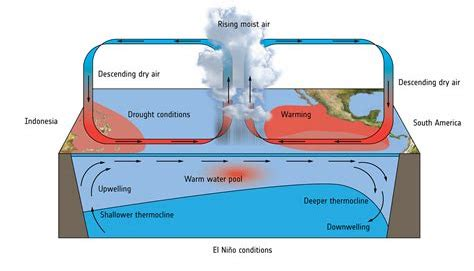
\includegraphics[width=\textwidth]{figures/example.jpg}
%       \caption{This is a very nice figure}
%       \label{fig:this}
%     \end{figure}
%   \end{columns}
% \end{frame}

\newcommand{\myfig}[3]{
  \begin{figure}
    \centering
    \includegraphics[width=\textwidth]{figures/#1}
    \caption{#2}
    \label{fig:#3}
  \end{figure}
}


\begin{document}

  \tikzstyle{process}=[circle, draw=process, fill=process!20, line width = 0.3mm]
  \tikzstyle{data}=[rectangle, draw=data, fill=data!20, line width = 0.3mm]

\maketitle

\section{Introduction}

\begin{frame}{Climate Change}

  \begin{columns}
    \column{0.6\textwidth}
    \begin{itemize}
    \item The earth is getting warmer. \citep{pachauri2014climate}
    \item Climate varies on different scales.
    \item Long-term trends and short-term noise.
    \item \alert{Forcing}: any external factor that affects climate.
      \begin{itemize}
      \item Greenhouse gasses
      \item Aerosols (natural: volcanic ash, artificial: smoke)
      \item Biomass burning
      \item Land use/cover (deforestation, desertification)
      \end{itemize}
    \end{itemize}
    \column{0.4\textwidth}
    \myfig{intro_fig_3.pdf}{Global mean land air temperature in GISSTEMP 4 dataset. \citep{gistemp2019giss} and \citep{lenssen2019improvements}}{this}
  \end{columns}
\end{frame}

\begin{frame}{El Niño (ENSO)}
  \begin{figure}
    \begin{columns}
      \column{0.5\textwidth}
      \begin{itemize}
      \item Warming and cooling of the Pacific Ocean.
      \item Affects human societies through temperature and rainfall. \citep{ropelewski1987global}
      \item May be affected by climate change.
      \end{itemize}
      \caption{Comparison of SST anomaly between 1975 La Niña event and 1997 El Niño event in HadISST 1 dataset. \citep{rayner2003global}}
      \column{0.5\textwidth}
      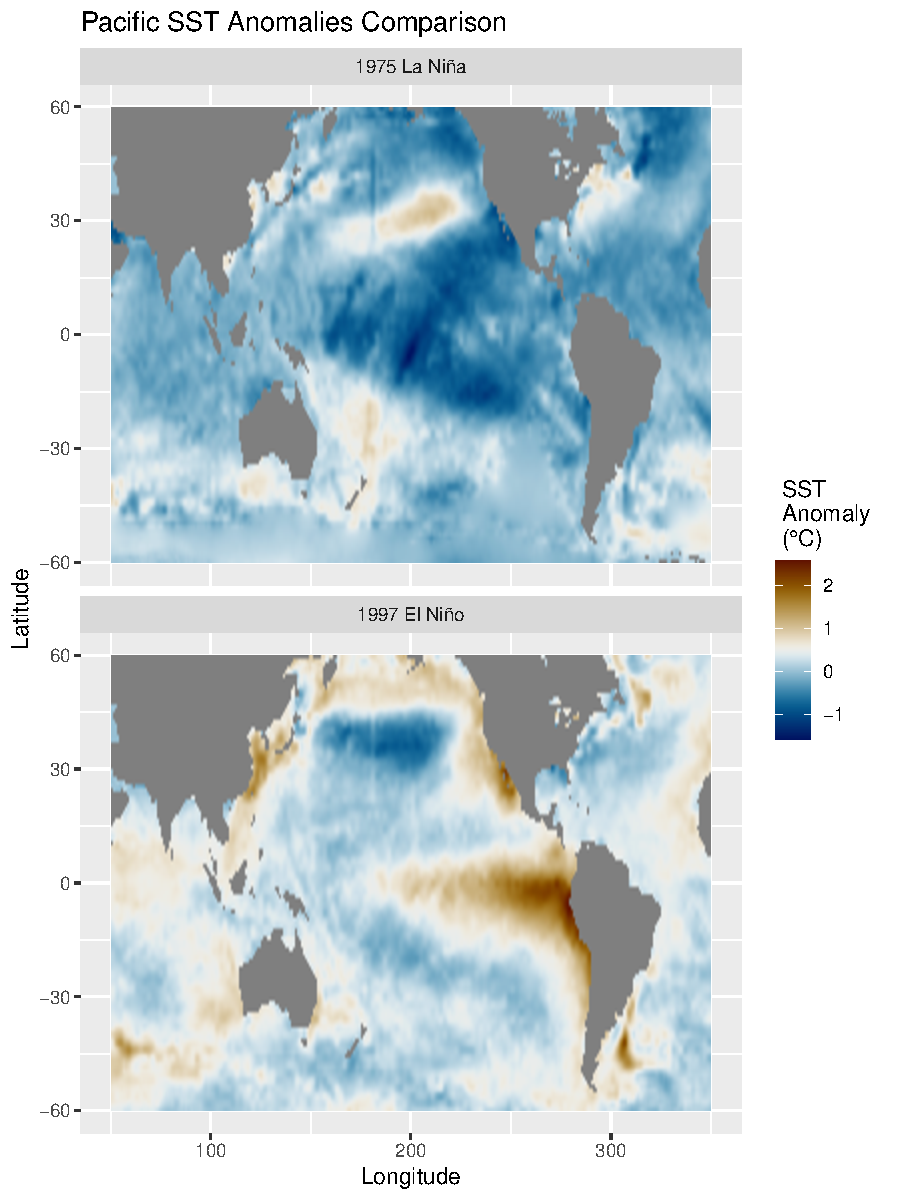
\includegraphics[width = \textwidth]{figures/intro_fig.pdf}
    \end{columns}
  \end{figure}
\end{frame}

\begin{frame}{Climate Simulation}
  \begin{itemize}
  \item Run climate simulation with predicted forcing levels as input.
  \item \alert{Ensemble:} set of repeated simulations.
  \end{itemize}
  \begin{tikzpicture}[node distance = 1.5in, line width = 0.5mm]
    \node (input) [data] {
      \begin{varwidth}{1.5in}
        Independent variables (forcing)
      \end{varwidth}};
    \node (model) [right of=input] [process] {
      \begin{varwidth}{\linewidth}
        Computer\\Simulation
      \end{varwidth}};
    \node (output) [right of=model] [data] {
      \begin{varwidth}{1.4in}
        Dependent variables (climatology)
      \end{varwidth}};
    \node (repeat) [above of=model, node distance = 1in] [process] {
      \begin{varwidth}{0.5in}
        Repeat
      \end{varwidth}};
    \draw [>->] (input) to (model);
    \draw [>->] (model) to (output);
    \draw [>->] (model) to [out = 50, in = 330] (repeat);
    \draw [>->] (repeat) to [out = 210, in = 130] (model);
  \end{tikzpicture}
\end{frame}

\begin{frame}{ENSO and Climate Change}
  \begin{itemize}
  \item ENSO changes over time \citep{lubbecke2014assessing}.
  \item ENSO responds to external forcing.
    \begin{itemize}
    \item Correlation between ENSO strength and sunspot activity \citep{emile2007nino}.
    \item Weakened ENSO during the Ice Age due to reduced CO$_2$ levels \citep{zhu2017reduced}.
    \end{itemize}
  \item Models show possible increasing ENSO activity in the future \citep{zheng2017response} and \citep{maher2018enso}.
  \item Factors other than CO$_2$ can affect ENSO.
    \begin{itemize}
    \item Ozone emission may reduce ENSO activity \citep{nowack2017role}
    \item Aerosol emission may reduce ENSO activity \citep{stevenson2017forced}
    \end{itemize}
  \end{itemize}
\end{frame}

\begin{frame}{Gap and Questions}
  Gap:
  \begin{itemize}
  \item Little research using a large ensemble to examine the effect of individual factors on ENSO.
  \item Considerable disagreement between studies on whether ENSO will strengthen or weaken due to global warming
  \end{itemize}
\end{frame}

\section{Data and Methods}

\begin{frame}{Role of Mentor and Student}
  \begin{columns}[t]
    \column{.5\textwidth}
    Mentor:
    \begin{itemize}
    \item Suggest future methods
    \item Conduct parallel analysis to complement student work
    \item Provide raw precollected data
    \item Interpret data produced by student
    \item Review student writing
    \end{itemize}
    \column{.5\textwidth}
    Student:
    \begin{itemize}
    \item Analyze data on computer
    \item Produce graphics for analysis and publication
    \item Write documentation
    \item Suggest interpretations of data
    \end{itemize}
  \end{columns}

\end{frame}

\begin{frame}{Model Setup}
  \begin{itemize}
  \item CESM1 \citep{kay2015community}
  \item CESM2 \citep{danabasoglu2020community}
  \item Observed forcing levels from 1850-2005
  \item Predicted forcing levels from 2005-2100
  \item Ensembles have 40 and 50 simulations respectively
  \item Control simulation with pre-1850 forcing levels
  \end{itemize}
\end{frame}

\begin{frame}{Measuring ENSO Intensity}
  \begin{tikzpicture}[node distance = 1.5in, line width = 0.5mm]
    \node [data] (input) {
      \begin{varwidth}{1.5in}
        External forcing
      \end{varwidth}};
    \node [process] (model) [right of=input] {
      \begin{varwidth}{\linewidth}
        CESM1\\and\\CESM2
      \end{varwidth}};
    \node [data] (output) [right of=model] {
      \begin{varwidth}{1.2in}
        Sea surface temperature (SST)
      \end{varwidth}};
    \node [data] (nino) [below of=input] {
      \begin{varwidth}{1.4in}
        Niño 3.4 index
      \end{varwidth}};
    \node [process] (variance) [right of=nino] {
      \begin{varwidth}{1.4in}
        Windowed\\variance
      \end{varwidth}};
    \node [data] (intensity) [right of=variance] {
      \begin{varwidth}{1.4in}
        ENSO intensity
      \end{varwidth}};
    \draw [->] (input) to (model);
    \draw [->] (model) to (output);
    \draw [->] (output) to [out = 270, in = 90] (nino);
    \draw [->] (nino) to (variance);
    \draw [->] (variance) to (intensity);
  \end{tikzpicture}
\end{frame}

\begin{frame}{Signal and Noise}
  \begin{columns}
    \column{0.3\textwidth}
    \begin{itemize}
      \item Butterfly effect
      \item Use ensemble mean to remove noise.
      \item The larger the ensemble, the less noise there is.
    \end{itemize}
    \column{0.7\textwidth}
    \myfig{variance_3.pdf}{ENSO intensity for each run of the CESM1 Large Ensemble}{variance_3}
  \end{columns}
\end{frame}

\begin{frame}{ENSO is Becoming Stronger}
  \begin{columns}
    \column{0.5\textwidth}
    \begin{itemize}
    \item Increase in ENSO intensity in both ensembles.
    \item Increase slows down in CESM1 and decreases in CESM2 after around 2050.
      \begin{itemize}
      \item May be caused by aerosol emissions.
      \end{itemize}
    \end{itemize}
    \column{0.5\textwidth}
    \myfig{ff_compare.pdf}{ENSO intensity ensemble mean and standard error for CESM1 and CESM2}{ff_compare}
  \end{columns}
\end{frame}

\begin{frame}{Single Forcing Ensembles}

\end{frame}

\begin{frame}{Influence of Aerosols and Greenhouse Gasses}

\end{frame}

\begin{frame}{Correlation With Ocean Temperature}

\end{frame}

\begin{frame}{Stratification}

\end{frame}

\begin{frame}{Wavelet Analysis}

\end{frame}

\begin{frame}{Power Spectrum}

\end{frame}

\section{Conclusion}

\begin{frame}{Conclusions}

\end{frame}

\begin{frame}{Discussion}

\end{frame}

\begin{frame}{Acknowledgments}
  \begin{itemize}
  \item This material is based upon work supported by the National Center for Atmospheric Research, which is a major facility sponsored by the National Science Foundation under Cooperative Agreement No. 1852977.
  \item Thank you to my teacher, my family, and my mentor!
  \item Software used: R, ncdf4, zoo, dplyr, ggplot2, WaveletComp, reshape2, nco.
  \end{itemize}
\end{frame}

\begin{frame}{References}
  \bibliographystyle{apalike}
  \fontsize{4pt}{5}\selectfont
  \bibliography{references.bib}
\end{frame}

\end{document}




%hi
